\documentclass[12pt]{article}
\usepackage[utf8]{inputenc}
\usepackage{float}
\usepackage{amsmath}


\usepackage[hmargin=3cm,vmargin=6.0cm]{geometry}
%\topmargin=0cm
\topmargin=-2cm
\addtolength{\textheight}{6.5cm}
\addtolength{\textwidth}{2.0cm}
%\setlength{\leftmargin}{-5cm}
\setlength{\oddsidemargin}{0.0cm}
\setlength{\evensidemargin}{0.0cm}

%misc libraries goes here
\usepackage{tikz}
\usetikzlibrary{automata,positioning}

\begin{document}

\section*{Student Information } 
%Write your full name and id number between the colon and newline
%Put one empty space character after colon and before newline
Full Name :  Kadir CETINKAYA\\
Id Number :  2036457 \\

% Write your answers below the section tags
\section*{Answer 1}

\subsection*{a.}
Let us define M as,
$$M=(K,\Sigma , \delta , s, H)\\$$
Let us define $\Sigma=\{x,\#,1,0,y\}\times\{0,1\}\times\{0,1\}$ where $x$ represents the
leftmost position symbol, $\#$ represents empty symbol and $y$ is the dummy
variable. The second element of the symbol tuple shows whether that cell 
had been initalized or not, $1$ and $0$ respectively. The last element
of the tuple represents whether the head for main tape is on that cell
or not, $1$ and $0$ respectively again.\\
\\
At the start our auxilary tape holds the row and column size in a unary
manner, always choosing $1$ as the second element of the tuple, $0$ as the last
element which will be irrelavant anyways for those elements, they are seperated from each other
by a blank symbol. $0$ represents the zero in unary manner. From now on
let us call these values $R$ and $C$, for the row and column size respectively.
And we fill main tape with the $(\#,0,0)$'s.\\
\\
Afterwards, of course putting a blank after the unary representation of $C$,
$R\times (C+1)$ symbols follow, all of which are $(y,1,0)$ except the first one
and every $(C+1)^{th}$ where the first element holds $(y,1,1)$ to represent the
head of the main tape is on that cell initially and $(\#,0,0)$ for every $(C+1)^{th}$
to represent the end of a row. Elements are ordered rowwise.
\\
$\delta$ is the transition function, which is a mapping,
$\delta: (K-H)\times(\Sigma\times\Sigma)\rightarrow K\times(\Sigma\cup\{\leftarrow,\rightarrow\})^2$\\
$s\in K$ is the start state and $H\subset K$ is the halting states of the machine.\\
\\
Definition of operations:\\
LA(Left Allocate): While performing this operation we look for the symbol which has $1$ in
last element of the tuple to find out the position of the head of the main tape then move head 
of the information tape left by one, if the symbol is a $(\#,0,0)$
then we need to allocate a new column, to do that we go to the starting of the auxilary tape
and go past the definiton of $R$ and $C$, afterwards we go right one by one and
every time we see a $(\#,0,0)$ we shift all content to the right by one and insert a
$(y,0,0)$, then we go back to the position which had $1$ in the last element of the tuple,
position of the head of the main tape and go left by one. So we are out of the if block now,
and we are sure that we are in the range of the main tape. We set second element of the current
symbol to $1$ to make sure it is allocated, if it is already allocated this does not change a thing
as we are not modifying the first element of the tuple, and we also set the last element of the
tuple to $1$ to move head of the main tape to that position, then we go right and set the
last element of the tuple to $0$ to make sure there is no ambiguity about the position of the
main tape's head. Then we increment $C$ by one, by shifting every element to the right
by one and inserting $(1,0,0)$ at the created position. Lastly, we go to the begining of the auxilary tape, and also we move main tape's
head to the left by one, if that value isn't initialized write $(y,1,1)$, otherwise just set its third
element to $1$, and set third element of the symbol at right to $0$.\\
\\
LB(Left Blank): While performing this operation we look for the symbol which has $1$ in
last element of the tuple to find out the position of the head of the main tape then move head 
of the information tape left by one, if the symbol is a $(\#,0,0)$
then we need to allocate a new column, to do that we go to the starting of the auxilary tape
and go past the definiton of $R$ and $C$, afterwards we go right one by one and
every time we see a $(\#,0,0)$ we shift all content to the right by one and insert a
$(y,0,0)$, then we go back to the position which had $1$ in the last element of the tuple,
position of the head of the main tape and go left by one. So we are out of the if block now,
and we are sure that we are in the range of the main tape. Different from the LA, we look at the
second element of the tuple, if it is a zero, we set it to $1$ to make sure it is allocated
and set first element of the tuple to $\#$, if it was already $1$ we do not perform that operation.
and we also set the last element of the tuple to $1$ to move head of the main tape to that position,
then we go right and set the last element of the tuple to $0$ to make sure there is no ambiguity about
the position of the main tape's head. T<hen we increment $C$ by one, by shifting every element to the right
by one and inserting $(1,0,0)$ at the created position. Lastly, we go to the begining of the auxilary tape, and also we move 
main tape's head to the left by one, if that value isn't initialized write $(\#,1,1)$, otherwise
just set its third element to $1$, and set third element of the symbol at right to $0$.\\
\\
RA(Right Allocate): While performing this operation we look for the symbol which has $1$ in
last element of the tuple to find out the position of the head of the main tape then move head 
of the information tape right by one, if the symbol is a $(\#,0,0)$
then we need to allocate a new column, to do that we go to the starting of the auxilary tape
and go past the definiton of $R$ and $C$, then we go right once more to get past the
first row's starting symbol, afterwards we go right one by one and
every time we see a $(\#,0,0)$, we go left by one and we shift all content to the right by one and insert a
$(y,0,0)$, then we go back to the position which had $1$ in the last element of the tuple,
position of the head of the main tape and go right by one. So we are out of the if block now,
and we are sure that we are in the range of the main tape. We set second element of the current
symbol to $1$ to make sure it is allocated, if it is already allocated this does not change a thing
as we are not modifying the first element of the tuple, and we also set the last element of the
tuple to $1$ to move head of the main tape to that position, then we go left and set the
last element of the tuple to $0$ to make sure there is no ambiguity about the position of the
main tape's head. Then we increment $C$ by one, by shifting every element to the right
by one and inserting $(1,0,0)$ at the created position. Lastly, we go to the begining of the auxilary tape, and also we move main tape's
head to the right by one, if that value isn't initialized write $(y,1,1)$, otherwise
just set its third element to $1$, and set third element of the symbol at left to $0$.\\
\\
RB(Right Blank): While performing this operation we look for the symbol which has $1$ in
last element of the tuple to find out the position of the head of the main tape then move head 
of the information tape right by one, if the symbol is a $(\#,0,0)$
then we need to allocate a new column, to do that we go to the starting of the auxilary tape
and go past the definiton of $R$ and $C$, then we go right once more to get past the first row's
starting symbol, afterwards we go right one by one and
every time we see a $(\#,0,0)$, we go left by one and we shift all content to the right by one and insert a
$(y,0,0)$, then we go back to the position which had $1$ in the last element of the tuple,
position of the head of the main tape and go right by one. So we are out of the if block now,
and we are sure that we are in the range of the main tape. Different from the RA, we look at the
second element of the tuple, if it is a zero, we set it to $1$ to make sure it is allocated
and set first element of the tuple to $\#$, if it was already $1$ we do not perform that operation.
and we also set the last element of the tuple to $1$ to move head of the main tape to that position,
then we go left and set the last element of the tuple to $0$ to make sure there is no ambiguity about
the position of the main tape's head. Then we increment $C$ by one, by shifting every element to the right
by one and inserting $(1,0,0)$ at the created position. Lastly, we go to the begining of the auxilary tape, and also we move 
main tape's head to the right by one, if that value isn't initialized write $(\#,1,1)$, otherwise
just set its third element to $1$, and set third element of the symbol at left to $0$.\\
\\
UA(Up Allocate): While performing this operation we look for the symbol which has $1$ in
last element of the tuple to find out the position of the head of the main tape then move head 
of the information tape to the left $C+1$ times to get to the cell above, if the symbol is a $(\#,0,0)$
then we need to allocate a new row, to do that we go left till we see a $(\#,0,0)$, then 
we shift all content to the right by $C+1$ to create new space for the row and insert $(y,0,0)$ to the
every new created area except the last one, insert a $(\#,0,0)$ to the last position to mark end of the new row.
Afterwards we go back then we go back to the position which had $1$ in the last element of the tuple,
position of the head of the main tape and go left $C+1$ times. So we are out of the if block now,
and we are sure that we are in the range of the main tape. We set second element of the current
symbol to $1$ to make sure it is allocated, if it is already allocated this does not change a thing
as we are not modifying the first element of the tuple, and we also set the last element of the
tuple to $1$ to move head of the main tape to that position, then we go right $C+1$ times and set the
last element of the tuple to $0$ to make sure there is no ambiguity about the position of the
main tape's head. then we increment $R$ by one, by shift every element to the right by one
and inserting $(1,0,0)$ at the created position. Lastly, we go to the begining of the auxilary tape
and also we move main tape's head to the up by one, if that value isn't initialized write $(y,1,1)$, otherwise
just set its third element to $1$, and set third element of the symbol at below to $0$.\\
\\
UB(Up Blank): While performing this operation we look for the symbol which has $1$ in
last element of the tuple to find out the position of the head of the main tape then move head 
of the information tape to the left $C+1$ times to get to the cell above, if the symbol is a $(\#,0,0)$
then we need to allocate a new row, to do that we go left till we see a $(\#,0,0)$, then 
we shift all content to the right by $C+1$ to create new space for the row and insert $(y,0,0)$ to the
every new created area except the last one, insert a $(\#,0,0)$ to the last position to mark end of the new row.
Afterwards we go back then we go back to the position which had $1$ in the last element of the tuple,
position of the head of the main tape and go left $C+1$ times. So we are out of the if block now,
and we are sure that we are in the range of the main tape. If the second element of the
current symbol is a $0$, then we set it to $1$ and also set the first element of the tuple to $\#$,
if it is a $1$ we do not perform that operation, then we set the last element of the
tuple to $1$ to move head of the main tape to that position, then we set the last element of the
tuple to $1$ to move head of the main tape to that position, then we go right $C+1$ times and set the
last element of the tuple to $0$ to make sure there is no ambiguity about the position of the
main tape's head. then we increment $R$ by one, by shift every element to the right by one
and inserting $(1,0,0)$ at the created position. Lastly, we go to the begining of the auxilary tape
and also we move main tape's head to the up by one, if that value isn't initialized write $(\#,1,1)$, otherwise
just set its third element to $1$, and set third element of the symbol at below to $0$.\\
\\
DA(Down Allocate): While performing this operation we look for the symbol which has $1$ in
last element of the tuple to find out the position of the head of the main tape then move head 
of the information tape to the right $C+1$ times to get to the cell below, if the symbol is a $(\#,0,0)$
then we need to allocate a new row, to do that we go right till we see a $(\#,0,0)$, then 
we insert $(y,0,0)$ to the right $C$ times and insert a $(\#,0,0)$ to mark the end of the new row,
afterwards we go back to the position which had $1$ in the last element of the tuple,
position of the head of the main tape and go right $C+1$ times. So we are out of the if block now,
and we are sure that we are in the range of the main tape. Then we set second element of the current symbol
to $1$, if it is already a $1$ this does not change anything, then we set the last element of the
tuple to $1$ to move head of the main tape to that position, then we go left $C+1$ times and set the
last element of the tuple to $0$ to make sure there is no ambiguity about the position of the
main tape's head. then we increment $R$ by one, by shift every element to the right by one
and inserting $(1,0,0)$ at the created position. Lastly, we go to the begining of the auxilary tape
and also we move main tape's head to the down by one, if that value isn't initialized write $(y,1,1)$, otherwise
just set its third element to $1$, and set third element of the symbol at above to $0$.\\
\\
DB(Down Blank): While performing this operation we look for the symbol which has $1$ in
last element of the tuple to find out the position of the head of the main tape then move head 
of the information tape to the right $C+1$ times to get to the cell below, if the symbol is a $(\#,0,0)$
then we need to allocate a new row, to do that we go right till we see a $(\#,0,0)$, then 
we insert $(y,0,0)$ to the right $C$ times and insert a $(\#,0,0)$ to mark the end of the new row,
afterwards we go back to the position which had $1$ in the last element of the tuple,
position of the head of the main tape and go right $C+1$ times. So we are out of the if block now,
and we are sure that we are in the range of the main tape. If the second element of the
current symbol is a $0$, then we set it to $1$ and also set the first element of the tuple to $\#$,
if it is a $1$ we do not perform that operation, then we set the last element of the
tuple to $1$ to move head of the main tape to that position, then we go left $C+1$ times and set the
last element of the tuple to $0$ to make sure there is no ambiguity about the position of the
main tape's head. then we increment $R$ by one, by shift every element to the right by one
and inserting $(1,0,0)$ at the created position. Lastly, we go to the begining of the auxilary tape
and also we move main tape's head to the down by one, if that value isn't initialized write $(\#,1,1)$, otherwise
just set its third element to $1$, and set third element of the symbol at above to $0$.\\
\\
T(Transpose access): While performing this operation, we go past $R$ and $C$ afterwards we look
for an element which has $1$ in last element of the tuple to find out the position of the head of the main
tape, while doing this every time we see a row start symbol, $(\#,0,0)$, we go the end of the main tape's
data holder, namely move $R*(C+1)$ positions to the right after the ending of $C$, and shift everything to
the right by one and insert $1$, so we are counting the row index of the main tape's header, let us call this $r$
from now on. After we found the symbol with $1$ in its last tuple element, we go to the left till we see
the row start symbol, $(\#,0,0)$, then we go right by one, and insert a one after the definition of $r$, again
by shifting everyting to the right by one, that way we count the column index of the head's position for main tape
lets call this $c$ from now on, we dothat untill we see the element with $1$ in its last tuple entry.
Then we rewind the auxilary tape to right after the definition of $C$, and we go right until we see $c$
times the row start symbol, after that we go right $r$ times unless we see a $(\#,0,0)$ symbol
which would imply we changed a row, but we should've stayed in the same row, if that happens we just clear
$r$ and $c$ and finish, otherwise we check the current symbol after going right $r$ times, if the second
element of the tuple is a $0$, it would mean that we are on a non-initalized cell so we would
clear $r$ and $c$ and finish again, if not we would set the last element of the tuple to $1$
and go to the symbol which is to the right of the begining $r*(c+1)$ times, and set its last tuple
to $0$ to make sure our main tape's head is pointing in the correct cell without ambiguity and we finish.
After we finish, if we've succeeded in changing the position in auxilary tape, move head of the main tape
to the $c,r$ also.
\\

\subsection*{b.}
In part a. we already simulated it almost for a TM with one tape, we just forget
about the operations we performed on main data tape, and perform nothing on
second tape of the new TM N, as it is not needed by our definition in part a.

\subsection*{c.}
Yes, it is. In part a. all of the operations were simulated on a semifinite one taped TM
all we need to do is delete the last sentences which moves main tapes head to the
corresponding position, we hold it's position in auxilary tape anyways, it is the
only part that keeps it from becoming a standard TM.



\section*{Answer 2}

\subsection*{a.}
$F=(K, \Sigma, \delta, s, H)$ where, $\Sigma = \{0,1,;,\#,x\}$ in which $1$
represents the unary ones, $0$ represents zero, $;$ is used for seperation
of input parameters $x, y$, $\#$ is the blank symbol and $x$ is the leftmost
position indicator. Since we are adopting the book notation, the first tape
is initially in the form ${x\#X;Y\#\#\#\#...}$ where $X$ and $Y$ stays for unary
representations of input variables and second tape is in the form ${x\#\#...}$
and we start in configuration ${(s, (x\underline{\#}w, x\underline{\#})}$.
Our transition funtion is a mapping from $(K-H)\times \Sigma^2$ to 
$K\times (\Sigma \cup \{\leftarrow, \rightarrow \})^2$. In the below
transition an arrow without any condition says that, if no other transition
is possible from that machine perform that one. $R,L,1,0,\#$ are the
basic turing machines which perform move head right, left; write 1, 0, \#
to the head's position respectively, $L_t,R_t$ are basic transition machines
which performs move left till you match character t and move right till you
match character t respectively. Also $X^k, X^{k,l}$ represents perform the
machine $X$'s operations on tape $k$ or $k,l$ respectively.

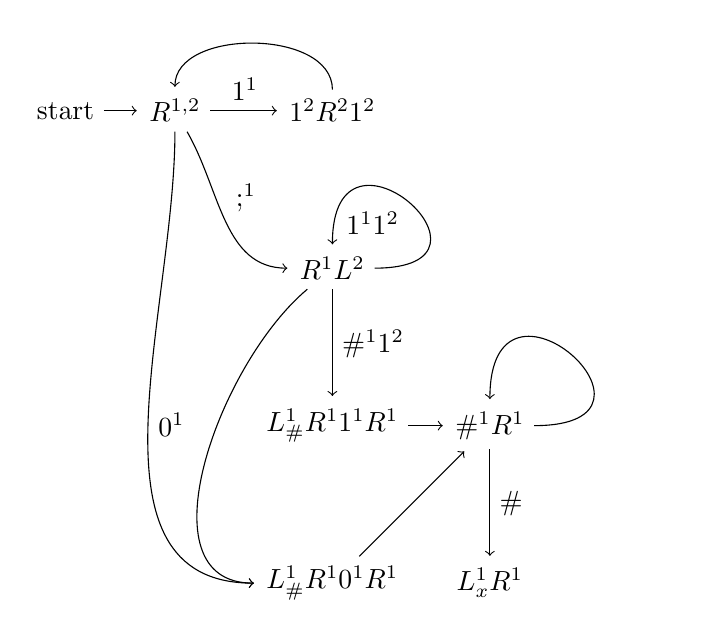
\begin{tikzpicture}[shorten >= 1pt, node distance=2cm, on grid, auto]
	\node[initial] (0) {$R^{1,2}$};
	\node (1) [right=of 0] {$1^2R^21^2$};
	\node (2) [below=of 1] {$R^1L^2$};
	\node (3) [below=of 2] {$L_\#^1R^11^1R^1$};
	\node (4) [below=of 3] {$L_\#^1R^10^1R^1$};
	\node (5) [right=of 3] {$\#^1R^1$};
	\node (6) [right=of 4] {$L_x^1R^1$};

	\path[->]
		(0) edge node {$1^1$} (1)
		(0) edge [in=180, out=300] node {$;^1$} (2)
		(0) edge [in=180, out=270] node {$0^1$} (4)
		(1) edge [in=90, out=90] node {} (0)
		(2) edge [in=90, out=0, loop] node {$1^11^2$} (2)
		(2) edge node {$\#^11^2$} (3)
		(2) edge [in=180, out=220] node {} (4)
		(3) edge node {} (5)
		(4) edge node {} (5)
		(5) edge [in=90, out=0, loop] node {} (5)
		(5) edge node {$\#$} (6);
\end{tikzpicture}

\subsection*{b.}
$G=(K, \Sigma, \delta, s, H)$ where, $\Sigma = \{0,1,\#,x\}$ in which $1$
represents the unary ones, $0$ represents zero, $\#$ is the blank symbol and 
$x$ is the leftmost position indicator. Since we are adopting the book notation, 
the first tape is initially in the form ${x\#X\#\#\#\#...}$ where $X$ stands for unary
representations of input variable and second tape is in the form ${x\#\#...}$
and we start in configuration ${(s, (x\underline{\#}w, x\underline{\#})}$.
Our transition funtion is a mapping from $(K-H)\times \Sigma^2$ to 
$K\times (\Sigma \cup \{\leftarrow, \rightarrow \})^2$. In the below
transition an arrow without any condition says that, if no other transition
is possible from that machine perform that one. $R,L,1,0,\#$ are the
basic turing machines which perform move head right, left; write 1, 0, \#
to the head's position respectively, $L_t,R_t$ are basic transition machines
which performs move left till you match character t and move right till you
match character t respectively. Also $X^k, X^{k,l}$ represents perform the
machine $X$'s operations on tape $k$ or $k,l$ respectively.

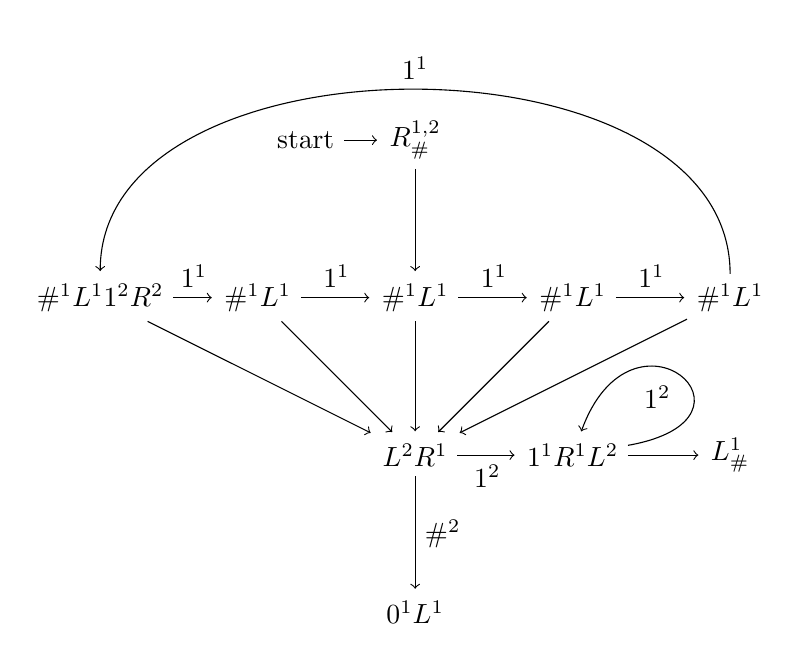
\begin{tikzpicture}[shorten >= 1pt, node distance=2cm, on grid, auto]
	\node[initial] (0) {$R_\#^{1,2}$};
	\node (2) [below=of 0] {$\#^1L^1$};
	\node (1) [left=of 2] {$\#^1L^1$};
	\node (5) [left=of 1] {$\#^1L^11^2R^2$};
	\node (3) [right=of 2] {$\#^1L^1$};
	\node (4) [right=of 3] {$\#^1L^1$};
	\node (6) [below=of 2] {$L^2R^1$};
	\node (7) [below=of 6] {$0^1L^1$};
	\node (8) [right=of 6] {$1^1R^1L^2$};
	\node (9) [right=of 8] {$L_\#^1$};

	\path[->]
		(0) edge node {} (2)
		(1) edge node {} (6)
		(2) edge node {} (6)
		(3) edge node {} (6)
		(4) edge node {} (6)
		(5) edge node {} (6)
		(1) edge node {$1^1$} (2)
		(2) edge node {$1^1$} (3)
		(3) edge node {$1^1$} (4)
		(4) edge [in=90, out=90] node [swap] {$1^1$} (5)
		(5) edge node {$1^1$} (1)
		(6) edge node {$\#^2$} (7)
		(6) edge node [swap] {$1^2$} (8)
		(8) edge [in=70, out=10, loop] node {$1^2$} (8)
		(8) edge node {} (9);
\end{tikzpicture}


\subsection*{c.}
$H=(K, \Sigma, \delta, s, H)$ where, $\Sigma = \{0,1,\#,x\}$ in which $1$
represents the unary ones, $0$ represents zero, $\#$ is the blank symbol and 
$x$ is the leftmost position indicator. Since we are adopting the book notation, 
the first tape is initially in the form ${x\#X\#\#\#\#...}$ where $X$ stands for unary
representations of input variable and second tape is in the form ${x\#\#...}$
and we start in configuration ${(s, x\underline{\#}w, x\underline{\#})}$.
Our transition funtion is a mapping from $(K-H)\times \Sigma^2$ to 
$K\times (\Sigma \cup \{\leftarrow, \rightarrow \})^2$. In the below
transition an arrow without any condition says that, if no other transition
is possible from that machine perform that one. $R,L,1,0,\#$ are the
basic turing machines which perform move head right, left; write 1, 0, \#
to the head's position respectively, $L_t,R_t$ are basic transition machines
which performs move left till you match character t and move right till you
match character t respectively. Also $X^k, X^{k,l}$ represents perform the
machine $X$'s operations on tape $k$ or $k,l$ respectively.

\begin{tikzpicture}[shorten >= 1pt, node distance=2cm, on grid, auto]
	\node[initial] (0) {$G^1$};
	\node (1) [right=of 0] {$R^1R^1$};
	\node (2) [right=of 1] {$L^1L^1$};
	\node (3) [below=of 1] {$L^1L^1R^21^2G^1R^1R^1$};
	\node (4) [below=of 3] {$L^1$};
	\node (7) [right=of 4] {$R^21^2$};
	\node (5) [right=of 7] {$1^1R^1L^2$};
	\node (6) [below=of 5] {$L_\#^1$};

	\path[->]
		(0) edge node {} (1)
		(1) edge node {} (3)
		(3) edge [in=30,out=0, loop] node {} (3)
		(4) edge node {} (7)
		(5) edge node {} (6)
		(1) edge node {$\#$} (2)
		(3) edge node {$\#$} (4)
		(4) edge node {$1^1$} (7)
		(4) edge [in=220,out=270] node {} (5)
		(7) edge node {} (5)
		(5) edge [in=90,out=0,loop] node {$1^2$} (5);
\end{tikzpicture}

It calculates the integer part of $log_5(2x)$.

\section*{Answer 3}
\subsection*{a.}
$M_f = (K, \Sigma, \delta, s, H)$, $K=\{s, q_0, q_1, q_2, y, n\}$, $H=\{y,n\}$,
$y$ is the accepting halt state, $n$ is the rejecting halt state.
$\Sigma = \{a,b,c,x,\#\}$, where $x$ represents tape start symbol and $\#$
represents blank symbol. $\delta : (K-H)\times \Sigma \rightarrow K\times 
(\Sigma \cup \{\leftarrow, \rightarrow\})$.
$$\delta(s,x)=(s, \rightarrow)$$
$$\delta(s,\#)=(q_0, \rightarrow)$$
$$\delta(s,a)=(n, \rightarrow)$$
$$\delta(s,b)=(n, \rightarrow)$$
$$\delta(s,c)=(n, \rightarrow)$$
$$\delta(q_0,x)=(n, \rightarrow)$$
$$\delta(q_0,\#)=(y, \rightarrow)$$
$$\delta(q_0,a)=(q_0, \rightarrow)$$
$$\delta(q_0,b)=(q_1, \rightarrow)$$
$$\delta(q_0,c)=(q_2, \rightarrow)$$
$$\delta(q_1,x)=(n, \rightarrow)$$
$$\delta(q_1,\#)=(y, \rightarrow)$$
$$\delta(q_1,a)=(n, \rightarrow)$$
$$\delta(q_1,b)=(q_1, \rightarrow)$$
$$\delta(q_1,c)=(q_2, \rightarrow)$$
$$\delta(q_2,x)=(n, \rightarrow)$$
$$\delta(q_2,\#)=(y, \rightarrow)$$
$$\delta(q_2,a)=(n, \rightarrow)$$
$$\delta(q_2,b)=(n, \rightarrow)$$
$$\delta(q_2,c)=(q_2, \rightarrow)$$

\subsection*{b.}
Let's have a turing machine M with 4 tapes, in its first tape we will
have the input string $w$. The second, third and fourth tapes will be filled
with blank initially. Then we can define our algorithm to decide whether
$w$ belongs to $L$ or not as follows:\\
\\
1. Read first character of the first tape, if it's not an $a$ reject
and halt, else go to step 2.\\
2. Write $111$ to the starting of the second tape.\\
3. Get head's of first and second tape to the begining.\\
4. Read from first and second tape, if character read from second tape is a $\#$
go to step 5, else if character read from first tape
is not an $a$, go to step 6, else shift both heads to right and go to step 4.\\
5. Write $1$ to the third tape and shift head to right, for each $1$ in the
second tape, write two $1$'s to the fourth tape, then copy contets of fourth
tape to the second tape. Get head of forth tape to the begining and go to step 4.\\
6. Get head of third tape to the begining, if character read from first tape is 
a $\#$ and character read from third tape is a $\#$ accept and halt.\\
7. Read from first and third tape, if character read from third tape is a $\#$
and character read from first tape is a $c$ go to step 8, else if character
read from third tape is a $1$ and character read from first tape is a $b$
shift both heads to the right and go to step 7, else reject and halt.\\
8. Clear second tape and get head of first and second tape to the begining.\\
9. Read character from the first tape, if it is an $a$ character write $1$ to the
second tape and move both heads to the right and go to step 9, else go to step 10.\\
10. Move head of the first tape to the right untill the character read is $c$.\\
11. Get head of third tape to the beginning.\\
12. Get head of second tape to the beggining.\\
13. If character read from second tape is a $\#$ then go to step 14, else if
character read from first tape is a $\#$ reject and halt, else move both heads
right and go to step 13.\\
14. Move head of third tape to the right, if character read is a $\#$ go to step 15,
else go to step 12.\\
15. If character read from first tape is a $\#$, accept and halt, else reject and halt.\\

\section*{Answer 4}

\subsection*{a.}
Since $L_2$ is finite, it must be a regular language.\\
Since the language $L_3$ can be recognized by a DPDA, it must be a language in DCFL,
moreover since, $L_3=\overline{L_1}\setminus L_2$ and $L_2$ is finite, $\overline{L_1}$
must also be a DCFL, which implies $L_1$ is also a DCFL.\\
Since $L_5$ can be recognized by a DTM, it must be a recursively enumerable language, moreover
since $\Sigma^*$ is the set of all words, any language's intersection with it is itself
therefore $L_5=\overline{L_3L_4}$. Since there exist a DTM recognizing that language, and also
since $L_3$ is a DCFL, we can easily construct a NTM that accepts $L_3L_4$. But, wait a second
we can both recognize $L_3L_4$ and $\overline{L_3L_4}$, so if we merge these two TM's we can
decide the language $\overline{L_3L_4}$, since every word in $\Sigma^*$ has to be in one of them,
at least one of the machines will always halt, there for the language $\overline{L_3L_4}$ is
decidable, so $L_5$ is a recursive language and so is $L_4$.\\
\\
$L_1$ is a DCFL.\\
$L_2$ is a regular language.\\
$L_3$ is a DCFL.\\
$L_4$ is recursive.\\
$L_5$ is recursive.\\

\subsection*{b.}
$L_6$ is also a recursive language, we can construct a new NTM M, that decides whether
a word is in $L_6$ or not. Firstly, since $L_3$ is a DCFL, so is $\overline{L_3}$, therefore
there exists a DPDA which recognizes it, which implies there exists a NTM, X, which decides
$\overline{L_3}$. Secondly, let us build a NTM, Y, which has 2-tapes, at the start it copies
its input in tape1 to tape2 in reverse order and then copie its second tape on to the first
tape, so it reverses its input. And lastly, since $L_5$ is a recursive language there exists
an NTM, Z, which decides whether a given word is in the language or not. So let us construct
our NTM, M, using those 3 TM's. Firstly for our given input we check whether X accepts the input
if so, we accept and halt. If not, first we send our word to Y and get reversed version of it
in our tape, afterwards we simply send it to Z, the result of Z is our result for the word.
We can show that like this:

\begin{tikzpicture}[shorten >= 1pt, node distance=4cm, on grid, auto]
	\node[initial] (0) {$X$};
	\node (1) [right=of 0] {$YZ$};
	\node (2) [above=of 1] {$\text{accept and halt}$};
	\node (3) [below=of 1] {$\text{reject and halt}$};

	\path[->]
		(0) edge node {$reject$} (1)
		(0) edge node {$accept$} (2)
		(1) edge node {$reject$} (3)
		(1) edge node [swap] {$accept$} (2);
\end{tikzpicture}


\end{document}

